\newcommand{\auditoriaid}{A04 -- Datos}
% Preambulo comun de las auditorias del informe E1 (revision_e1/)
\documentclass[11pt,a4paper]{article}
\usepackage[utf8]{inputenc}
\usepackage[T1]{fontenc}
\usepackage[spanish,es-noshorthands]{babel}
\usepackage{lmodern}
\usepackage{microtype}
% Sin patrones de guionado en espanol en esta instalacion (ver A10): se
% desactiva el guionado automatico para evitar cortes con reglas del ingles.
\hyphenpenalty=10000
\exhyphenpenalty=10000
\usepackage[a4paper,margin=2.2cm]{geometry}
\usepackage{booktabs,array,longtable}
\usepackage{graphicx,caption,subcaption}
\usepackage{xcolor}
\usepackage{enumitem}
\usepackage{fancyhdr}
\usepackage{amsmath}
\usepackage{tikz}
\usetikzlibrary{arrows.meta,positioning}
\usepackage{natbib}
\usepackage{xurl}
\usepackage[hidelinks]{hyperref}
\urlstyle{tt}
\newcommand{\archivo}[1]{\url{#1}}
\newcolumntype{L}[1]{>{\raggedright\arraybackslash}p{#1}}
\definecolor{alta}{RGB}{180,30,30}
\definecolor{media}{RGB}{200,120,0}
\definecolor{baja}{RGB}{60,110,160}
\definecolor{cajafondo}{RGB}{245,247,250}
\newcommand{\sevA}{\textcolor{alta}{\textbf{Alta}}}
\newcommand{\sevM}{\textcolor{media}{\textbf{Media}}}
\newcommand{\sevB}{\textcolor{baja}{\textbf{Baja}}}
\setlength{\parskip}{0.35em}
\setlength{\emergencystretch}{3em}
\setlength{\parindent}{0pt}
\pagestyle{fancy}
\fancyhf{}
\fancyhead[L]{\small Auditoría del Informe del Entregable~1 -- \auditoriaid}
\fancyhead[R]{\small \thepage}
\renewcommand{\headrulewidth}{0.4pt}
% Entorno de hallazgos: ID | Severidad | Ubicacion | Hallazgo y evidencia | Correccion
\newenvironment{hallazgos}{%
\small
\begin{longtable}{@{}L{1.15cm}L{1.25cm}L{1.9cm}L{6.0cm}L{\dimexpr\textwidth-10.3cm-10.6\tabcolsep\relax}@{}}
\toprule
\textbf{ID} & \textbf{Sev.} & \textbf{Ubicación} & \textbf{Hallazgo y evidencia} & \textbf{Corrección aplicada} \\
\midrule\endfirsthead
\toprule
\textbf{ID} & \textbf{Sev.} & \textbf{Ubicación} & \textbf{Hallazgo y evidencia} & \textbf{Corrección aplicada} \\
\midrule\endhead
\bottomrule\endfoot
}{\end{longtable}}
% Macros compartidas con el informe revisado (las secciones propuestas las usan)
% Macros compartidas entre el informe revisado y las auditorias.
% Cifras verificadas contra los archivos del repositorio (ver A01/A04/A07):
\newcommand{\nUniverso}{102}   % source_id CMIP6 con tos/Omon en ESGF (00b, model_availability_priority.csv)
\newcommand{\nSeed}{41}        % publican los cuatro experimentos (config/models_seed_cmip6.csv)
\newcommand{\nSel}{40}         % completos + QC PASS (models_inventory_final.csv)
\newcommand{\nComb}{160}       % combinaciones modelo-experimento PASS (qc_report.csv)
\newcommand{\nNoEnc}{44}       % config/models_no_encontrado_44.csv
\newcommand{\nParcial}{18}     % 102 - 40 - 44
% Fecha de la portada: fija (no \today), editable en un solo lugar.
\newcommand{\fechaentrega}{28 de septiembre de 2026}
% Estado de codigo que documenta el E1 (antes de los cambios del E2)
\newcommand{\commitEone}{\texttt{8ee6184}}

% En las auditorias el texto propuesto se muestra fuera del informe: las
% referencias cruzadas se imprimen con el nombre de la seccion destino.
\makeatletter
\def\etq#1#2{\expandafter\def\csname etq@#1\endcsname{#2}}
\etq{sec:resumen}{Resumen}
\etq{sec:alcance}{Alcance}
\etq{sec:marco}{Revisión científica}
\etq{sec:antecedentes}{Antecedentes}
\etq{sec:referencias}{Literatura sobre TOE}
\etq{tab:referencias}{bibliografía TOE}
\etq{sec:similitudes}{Niño~3.4 frente a Niño~1+2}
\etq{sec:toe_metodos}{Elección de los métodos de TOE}
\etq{tab:metodos_toe}{métodos TOE}
\etq{eq:szabo_signal}{ecuación señal M1}
\etq{eq:szabo_V}{ecuación V(t)}
\etq{eq:szabo_T}{ecuación T(t)}
\etq{eq:szabo_toe}{ecuación TOE M1}
\etq{eq:tod}{ecuación ToD}
\etq{sec:datos}{Datos}
\etq{fig:cmip6_contribution}{contribución institucional}
\etq{sec:tabla_modelos}{Modelos seleccionados}
\etq{tab:modelos}{modelos}
\etq{sec:desviacion}{Selección de modelos}
\etq{sec:dominios_periodos}{Dominios y periodos}
\etq{fig:region_nino}{regiones Niño}
\etq{sec:arquitectura}{Arquitectura del pipeline}
\etq{fig:flujograma}{Flujograma}
\etq{sec:scripts}{Descripción de los pasos}
\etq{sec:paso00b}{Paso 00b}
\etq{sec:paso01}{Paso 01}
\etq{sec:paso02}{Paso 02}
\etq{sec:paso04}{Paso 04}
\etq{sec:paso05}{Paso 05}
\etq{sec:paso06}{Paso 06}
\etq{sec:paso07}{Paso 07}
\etq{sec:reporte}{Reporte de estado}
\etq{sec:resultados}{Resultados}
\etq{fig:qc}{matriz de estado}
\etq{tab:cuentas}{conteo de modelos}
\etq{fig:mapas2d}{mapas 2D}
\etq{fig:series}{series}
\etq{fig:boxplot}{boxplots}
\etq{sec:roadmap}{Próximos pasos}
\etq{tab:roadmap}{próximos pasos}
\etq{sec:conclusiones}{Conclusiones}
\etq{sec:recomendaciones}{Recomendaciones}
\makeatother

\makeatletter
\AtBeginDocument{\renewcommand{\ref}[1]{\@ifundefined{etq@#1}{\textit{[#1]}}{\textit{\csname etq@#1\endcsname}}}}
\makeatother
% Texto propuesto: secciones degradadas un nivel y en caja
\newenvironment{propuesto}{%
  \par\medskip\noindent\textcolor{baja}{\rule{\textwidth}{0.8pt}}\par
  \noindent{\small\textbf{Inicio del texto propuesto para el informe revisado}}\par\medskip
  \begingroup
  \let\section\subsection\let\subsection\subsubsection\let\subsubsection\paragraph
}{%
  \endgroup
  \par\noindent{\small\textbf{Fin del texto propuesto}}\par
  \noindent\textcolor{baja}{\rule{\textwidth}{0.8pt}}\par\medskip}
% Recuadro de actualizacion posterior (decisiones del autor)
\newcommand{\actualizacion}[1]{\par\medskip\noindent\fcolorbox{media}{media!8}{\parbox{\dimexpr\linewidth-2\fboxsep-2\fboxrule\relax}{\small\textbf{Actualización del 29-09-2026 (decisiones del autor).} #1}}\par\medskip}

\graphicspath{{../}}
\begin{document}

\begin{center}
{\Large\bfseries Auditoría A04: Datos (fuentes, modelos, selección, dominios y periodos)}\\[0.4em]
{\normalsize Informe del Entregable~1, Sección~4 (\texttt{informe\_e1\_smnv3.tex}, commit \texttt{330fd2e})}\\[0.2em]
{\small Revisión: \fechaentrega}
\end{center}

\section{Objeto}

Se audita la Sección~4 completa: fuentes de datos, Figura de contribución institucional, Cuadro de los 40 modelos, ``Selección inicial de modelos'' y ``Dominios oceanográficos y periodos''. Los números se recalcularon desde los CSV del repositorio. Las figuras se contrastaron con la configuración del estado E1 (\texttt{git show 8ee6184:config/domains.yaml}) y con los archivos que efectivamente enlaza \archivo{informe/figuras/}.

\actualizacion{El informe describe la ventana de descarga vigente (0°--360°, 30°S--30°N), ampliada para el índice RONI y el índice $W$ del ToD, en lugar de la ventana original del E1. El mapa de regiones y los mapas 2D se regeneraron para toda esa ventana; el mapa de regiones pasó a una proyección cilíndrica centrada en Niño~3.4 entre 60°S y 60°N, para que la franja verde se vea rodeando el globo. Las figuras regeneradas con la ventana del E1 que se describen en la sección~4 de esta auditoría quedan solo como registro.}

\section{Verificaciones realizadas}

\begin{itemize}[leftmargin=1.2em]
\item \textbf{Cuadro de modelos.} Las 40 filas se cruzaron con \archivo{models_inventory_final.csv} (mismo conjunto) y con \archivo{informe/model_registry.csv}: coinciden código, institución, realización y resolución de cada fila. Distribución: 30 modelos con \texttt{r1i1p1f1}; 24 instituciones; 15 países; resoluciones nominales de 25\,km (2), 50\,km (1), 100\,km (24), 111\,km (4) y 250\,km (9).
\item \textbf{Modelos de \citet{bruno2023}.} Se extrajeron los 53 nombres de su Tabla~1 (ver A02-4). Los 53 están en el universo de 102; 32 están entre los 40 seleccionados; de los 21 restantes, 16 no publican \texttt{ssp245} o \texttt{ssp585} en ESGF y 5 solo carecen de \texttt{ssp370}.
\item \textbf{Efecto de exigir \texttt{ssp370}.} Sobre \archivo{model_availability_priority.csv}: 49 modelos publican \texttt{historical}+\texttt{ssp245}+\texttt{ssp585}; 8 no publican \texttt{ssp370} (CIESM, EC-Earth3-CC, FIO-ESM-2-0, GFDL-CM4, GISS-E2-1-G-CC, HadGEM3-GC31-LL, KIOST-ESM, NESM3). El requisito del escenario intermedio reduce el conjunto de 49 a 41.
\item \textbf{Figuras.} \archivo{informe/figuras/} contiene \emph{enlaces simbólicos} a \archivo{figures/}, carpeta no versionada que se regenera en cada corrida. Tras la corrida del 22-09 con la ventana ampliada para el E2 (\texttt{79a9786}), el mapa de regiones y los mapas 2D del PDF muestran 0°--360°, 30°S--30°N, y no la ventana que describe el texto. Se regeneraron con el código del E1 (sección~4).
\item \textbf{ERSSTv5.} URL de descarga en el Paso~03 del E1: \archivo{https://downloads.psl.noaa.gov/Datasets/noaa.ersst.v5/sst.mnmean.nc}; recorte con \texttt{sellonlatbox} y \texttt{selvar,sst}. Coincide con el texto.
\end{itemize}

\section{Hallazgos}

\begin{hallazgos}
A04-1 & \sevA & Figura de contribución & Imagen externa, no generada por el \emph{pipeline} (lo dice el README), sobre un mapa base comercial y sin fuente citada. Muestra banderas de países que no tienen modelos entre los 40 seleccionados (Brasil, Sudáfrica, Arabia Saudita, Chipre, Nueva Zelanda, entre otros), mientras el pie afirma que es la contribución ``al conjunto CMIP6 finalmente consolidado''. & Se reemplaza por una figura reproducible (\archivo{revision_e1/trabajo/fig_contribucion.py}): modelos seleccionados por país, con sus instituciones. \\
A04-2 & \sevA & 4.3, Selección & ``de los 52 \texttt{source\_id} distintos citados en \citet{bruno2023}, 34 coinciden \ldots, 16 más \ldots\ en \archivo{models_missing_from_esgf.csv} \ldots\ y 37 de los 52 terminaron \ldots\ en el inventario final''. Incoherente en sí mismo (37 en el inventario, pero solo 34 en el \emph{seed} del que sale el inventario) y contra los datos: 53 modelos, 32 seleccionados. \archivo{models_missing_from_esgf.csv} tiene 17 filas, y 3 de ellas ya están en el \emph{seed} (archivo desactualizado). & Cifras recalculadas: 53 / 102 / 32 / 21. \\
A04-3 & \sevA & 4.3, Selección & ``102 modelos (46 del barrido inicial más 56 citados en la literatura, verificados con \texttt{00c})'' (ver A01-1). & Universo = 102 modelos con \texttt{tos}/\texttt{Omon} en ESGF. \\
A04-4 & \sevA & 4.3 y 4.4 & No se informa que exigir \texttt{ssp370}, escenario no requerido por el TdR, reduce el conjunto de 49 a 41 modelos. Es una decisión metodológica con costo real para SSP2-4.5/5-8.5 y el lector debe conocerla. & Párrafo neutro con la cifra y la vía para reincorporar esos 8 modelos (ver A08). \\
A04-5 & \sevA & Fig.~\ref{fig:region_nino} y Fig.~\ref{fig:mapas2d} & El PDF compilado muestra la ventana del E2 (30°S--30°N, global) por los enlaces simbólicos, aunque el texto describe 100°E--70°O, 20°S--20°N. & Figuras regeneradas; en el informe revisado son archivos reales. \textit{Actualización 29-09: se usa la ventana vigente y el texto se ajustó a ella.} \\
A04-6 & \sevM & Pie del cuadro & ``Resolución \ldots\ la más gruesa entre las que publican los cuatro experimentos (Sección \texttt{sec:desviacion}), no la resolución final \ldots\ (ésa es siempre la de ERSSTv5)''. Correcto, pero con paréntesis anidados y guiones que dificultan la lectura. & Pie reescrito en oraciones cortas. \\
A04-7 & \sevM & 4.2 & El informe dice que el código se asignó ``alfabéticamente''. Verificado: el orden es el de \texttt{sorted()} de Python, que separa mayúsculas y minúsculas (CNRM antes que CanESM). Correcto como orden estable, no como orden alfabético estricto. & Se mantiene ``alfabéticamente'' (convención del registro); se anota aquí la sutileza. \\
A04-8 & \sevM & 4.2 & No explica por qué 10 modelos no usan \texttt{r1i1p1f1}. & Una frase: variante común a los cuatro experimentos cuando \texttt{r1i1p1f1} no los cubre. \\
A04-9 & \sevB & 4.1 & ``La Figura \ldots\ ilustra la contribución institucional internacional'': redundante, y su pie remitía a la Sección~3.3 por un argumento de sesgo estructural. & El argumento se deja en el pie de la figura nueva, sin remisión. \\
A04-10 & \sevB & 4.4 & Tres líneas en blanco consecutivas en el \texttt{.tex} y un párrafo huérfano (``La Figura~\ldots\ ubica ambas cajas'') entre la figura y los periodos. & Se elimina. \\
A04-11 & \sevB & Título 4.3 & ``Selección inicial de modelos'' describe la selección final completa, no una inicial. & ``Selección de modelos''. \\
A04-12 & -- & 4.4 & Verificado sin cambios: cajas Niño~3.4 (190°--240°, 5°S--5°N) y Niño~1+2 (270°--280°, 10°S--0°); ventana del E1 100°--290°, 20°S--20°N; periodos 1981--2014, 2036--2065, 2071--2100; descarga 1850--2100. & Se conservan. \\
\end{hallazgos}

\section{Figuras regeneradas con el código del E1}

Se extrajo \texttt{scripts/} y \texttt{config/} del commit \texttt{8ee6184} a \archivo{revision_e1/trabajo/e1_snapshot/}, con enlaces a \archivo{data/} e \archivo{informe/} del repositorio. El mapa de regiones se regeneró con el script original, que lee la ventana del E1. Los mapas 2D se regeneraron recortando el dato procesado a 100°--290°, 20°S--20°N antes de graficar. Recortar es equivalente a la corrida del E1, porque la grilla de destino (ERSSTv5) y la máscara de cada punto son las mismas: la ventana solo cambia la extensión. Las demás figuras del informe (matriz de estado, series y \emph{boxplots}) dependen de las cajas, no de la ventana, y se copiaron como archivos reales.

\begin{figure}[h]
\centering
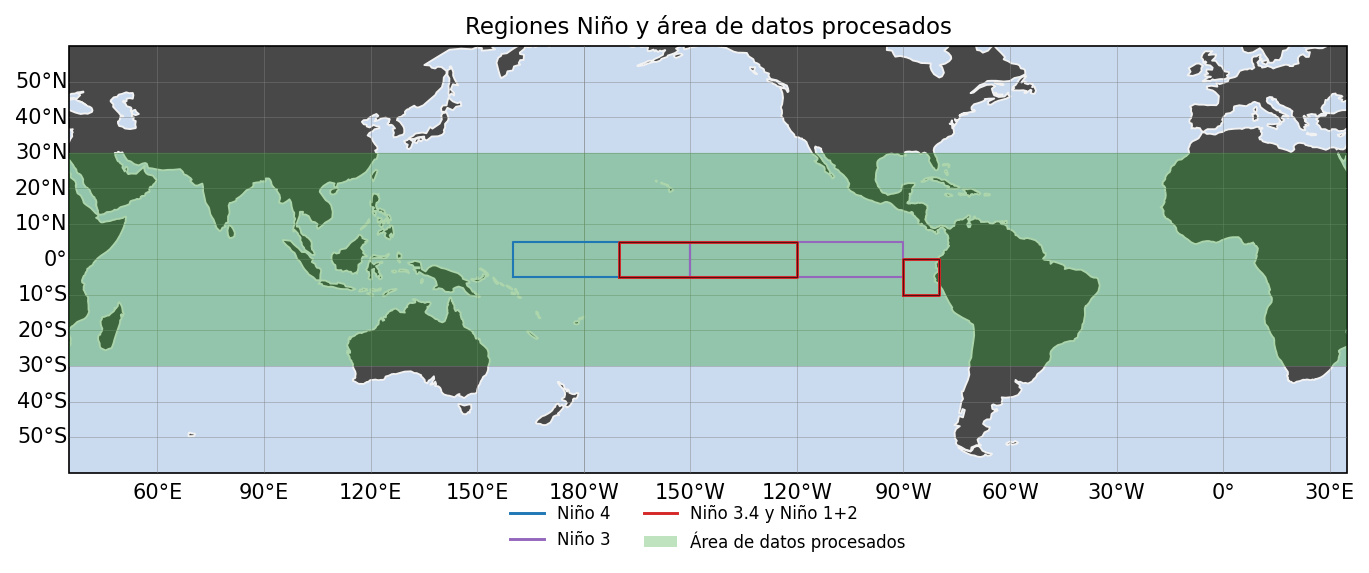
\includegraphics[width=0.85\textwidth]{figuras/region_nino_proj.png}
\caption{Mapa de regiones regenerado con la ventana del E1 (comparar con la ventana global del PDF actual).}
\end{figure}

\section{Extensión}

Original: 1599 palabras (incluido el cuadro). Propuesto: 1456 
palabras.

\section{Texto propuesto}

\begin{propuesto}
% ============================================================
\section{Datos}
\label{sec:datos}
% ============================================================

Se usan dos fuentes. La primera son las salidas de los modelos CMIP6 para la variable \texttt{tos} (TSM, tabla CMOR \texttt{Omon}), obtenidas de la federación ESGF (\emph{Earth System Grid Federation}) y, de forma complementaria, del Copernicus Climate Data Store (CDS). La segunda es ERSSTv5 (\emph{Extended Reconstructed Sea Surface Temperature}, versión~5) de NOAA, descargada de NOAA PSL, que es la referencia observacional única de todo el \emph{pipeline}. La Figura~\ref{fig:cmip6_contribution} muestra la procedencia institucional de los 40 modelos seleccionados.

\begin{figure}[htbp]
\centering
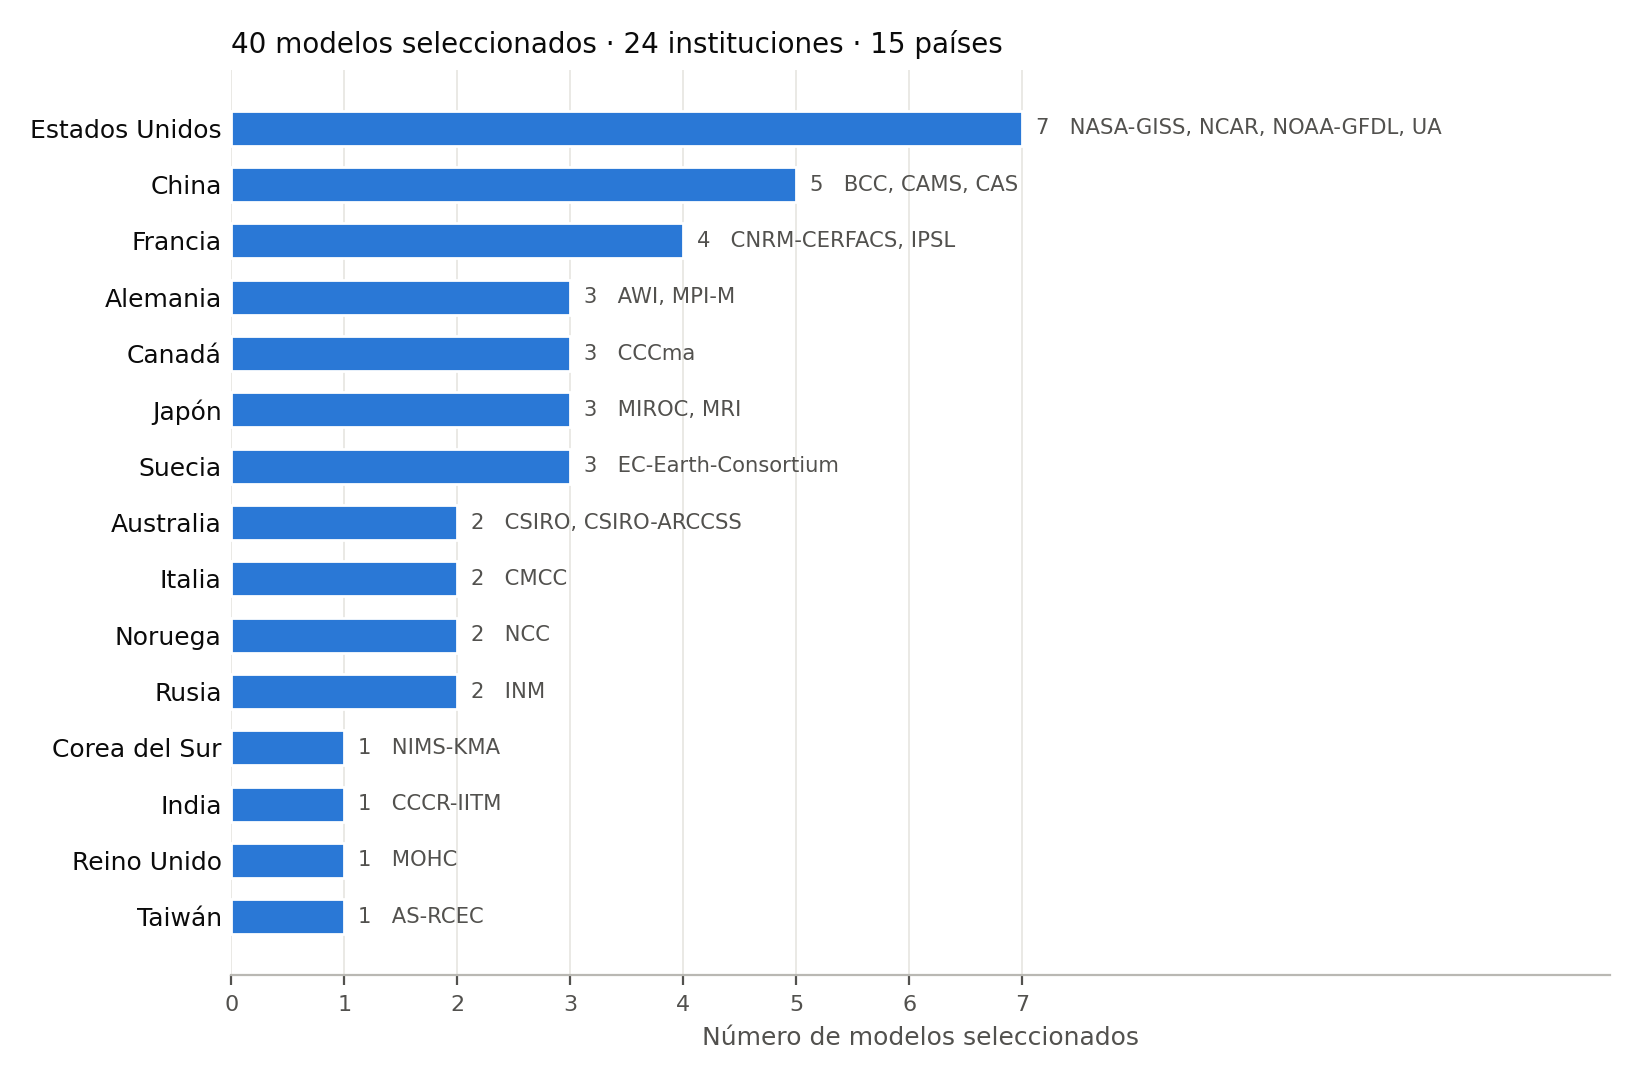
\includegraphics[width=0.92\textwidth]{figuras/contribucion_paises.png}
\caption[Modelos CMIP6 seleccionados por país e institución de origen.]{Modelos CMIP6 seleccionados por país de la institución que los publica, con las instituciones de cada país (fuente: \archivo{informe/model_registry.csv} y \archivo{data/processed/models_inventory_final.csv}). La diversidad de centros de modelado importa para la incertidumbre de modelo: modelos de un mismo centro comparten componentes y, con mayor probabilidad, sesgos estructurales (por ejemplo, la lengua fría o la doble ZCIT del Pacífico oriental), lo que puede reducir artificialmente la dispersión entre modelos.}
\label{fig:cmip6_contribution}
\end{figure}

\subsection{Modelos CMIP6 seleccionados}
\label{sec:tabla_modelos}

El Cuadro~\ref{tab:modelos} lista los 40 modelos seleccionados, con los cuatro experimentos completos y aprobados en el control de calidad (Sección~\ref{sec:resultados}). Cada modelo se identifica con un código \texttt{M001}--\texttt{M102}, asignado alfabéticamente sobre el universo completo de 102 candidatos (\archivo{informe/model_registry.csv}), de modo que un mismo código designa siempre al mismo modelo en cualquier figura o corrida. Las columnas siguen el orden habitual de las tablas de intercomparación CMIP6: primero la identidad del modelo (código, nombre, institución y país) y después sus especificaciones técnicas (miembro de ensamble y resolución nominal). No se incluye una columna de experimentos porque los 40 modelos tienen los mismos cuatro; la disponibilidad por experimento del universo completo se muestra en la Figura~\ref{fig:qc}.

\begingroup\small
\begin{longtable}{@{}L{1.3cm}L{2.9cm}L{3.5cm}L{2.5cm}L{2.1cm}L{\dimexpr\textwidth-12.3cm-10\tabcolsep\relax}@{}}
\caption[Modelos CMIP6 seleccionados: código, institución, país, realización y resolución nominal.]{Modelos CMIP6 seleccionados. Código: identificador estable \texttt{M001}--\texttt{M102}. Institución: \archivo{institution_id} de CMIP6. País: derivado del vocabulario controlado oficial de CMIP6 (\archivo{WCRP-CMIP/CMIP6_CVs}); para consorcios multinacionales como EC-Earth es el país de la sede administrativa. Realización: \archivo{variant_label} común a los cuatro experimentos. Resolución: \archivo{nominal_resolution} de la variante de grilla descargada, la más gruesa entre las que cubren los cuatro experimentos (Sección~\ref{sec:desviacion}); tras el regrillado del Paso~04 todos los modelos comparten la grilla de ERSSTv5 ($\sim$2°).}
\label{tab:modelos} \\
\toprule
\textbf{Código} & \textbf{Modelo} & \textbf{Institución} & \textbf{País} & \textbf{Realización} & \textbf{Resolución} \\
\midrule
\endfirsthead
\toprule
\textbf{Código} & \textbf{Modelo} & \textbf{Institución} & \textbf{País} & \textbf{Realización} & \textbf{Resolución} \\
\midrule
\endhead
\bottomrule
\endfoot
M001 & ACCESS-CM2 & CSIRO-ARCCSS & Australia & r1i1p1f1 & 250\,km \\
M002 & ACCESS-ESM1-5 & CSIRO & Australia & r1i1p1f1 & 250\,km \\
M007 & AWI-CM-1-1-MR & AWI & Alemania & r1i1p1f1 & 25\,km \\
M010 & BCC-CSM2-MR & BCC & China & r1i1p1f1 & 100\,km \\
M012 & CAMS-CSM1-0 & CAMS & China & r1i1p1f1 & 100\,km \\
M013 & CAS-ESM2-0 & CAS & China & r1i1p1f1 & 100\,km \\
M017 & CESM2 & NCAR & Estados Unidos & r1i1p1f1 & 111\,km \\
M019 & CESM2-WACCM & NCAR & Estados Unidos & r1i1p1f1 & 111\,km \\
M023 & CMCC-CM2-SR5 & CMCC & Italia & r1i1p1f1 & 100\,km \\
M025 & CMCC-ESM2 & CMCC & Italia & r1i1p1f1 & 100\,km \\
M026 & CNRM-CM6-1 & CNRM-CERFACS & Francia & r1i1p1f2 & 100\,km \\
M027 & CNRM-CM6-1-HR & CNRM-CERFACS & Francia & r1i1p1f2 & 25\,km \\
M028 & CNRM-ESM2-1 & CNRM-CERFACS & Francia & r1i1p1f2 & 100\,km \\
M029 & CanESM5 & CCCma & Canadá & r1i1p1f1 & 100\,km \\
M030 & CanESM5-1 & CCCma & Canadá & r1i1p1f1 & 100\,km \\
M031 & CanESM5-CanOE & CCCma & Canadá & r1i1p2f1 & 100\,km \\
M038 & EC-Earth3 & EC-Earth-Consortium & Suecia & r1i1p1f1 & 100\,km \\
M043 & EC-Earth3-Veg & EC-Earth-Consortium & Suecia & r1i1p1f1 & 100\,km \\
M044 & EC-Earth3-Veg-LR & EC-Earth-Consortium & Suecia & r1i1p1f1 & 100\,km \\
M051 & FGOALS-f3-L & CAS & China & r1i1p1f1 & 100\,km \\
M052 & FGOALS-g3 & CAS & China & r1i1p1f1 & 100\,km \\
M056 & GFDL-ESM4 & NOAA-GFDL & Estados Unidos & r1i1p1f1 & 111\,km \\
M057 & GISS-E2-1-G & NASA-GISS & Estados Unidos & r1i1p3f1 & 250\,km \\
M059 & GISS-E2-1-H & NASA-GISS & Estados Unidos & r1i1p3f1 & 250\,km \\
M060 & GISS-E2-2-G & NASA-GISS & Estados Unidos & r1i1p3f1 & 250\,km \\
M069 & IITM-ESM & CCCR-IITM & India & r1i1p1f1 & 250\,km \\
M070 & INM-CM4-8 & INM & Rusia & r1i1p1f1 & 100\,km \\
M071 & INM-CM5-0 & INM & Rusia & r1i1p1f1 & 100\,km \\
M074 & IPSL-CM6A-LR & IPSL & Francia & r1i1p1f1 & 100\,km \\
M077 & KACE-1-0-G & NIMS-KMA & Corea del Sur & r1i1p1f1 & 250\,km \\
M079 & MCM-UA-1-0 & UA & Estados Unidos & r1i1p1f2 & 250\,km \\
M081 & MIROC-ES2L & MIROC & Japón & r1i1p1f2 & 111\,km \\
M082 & MIROC6 & MIROC & Japón & r1i1p1f1 & 100\,km \\
M084 & MPI-ESM1-2-HR & MPI-M & Alemania & r1i1p1f1 & 50\,km \\
M085 & MPI-ESM1-2-LR & MPI-M & Alemania & r1i1p1f1 & 250\,km \\
M087 & MRI-ESM2-0 & MRI & Japón & r1i1p1f1 & 100\,km \\
M094 & NorESM2-LM & NCC & Noruega & r1i1p1f1 & 100\,km \\
M095 & NorESM2-MM & NCC & Noruega & r1i1p1f1 & 100\,km \\
M097 & TaiESM1 & AS-RCEC & Taiwán & r1i1p1f1 & 100\,km \\
M100 & UKESM1-0-LL & MOHC & Reino Unido & r1i1p1f2 & 100\,km \\
\end{longtable}
\endgroup

La resolución nominal es una categoría del vocabulario controlado de CMIP6, no una medida continua, y se consulta en el índice de ESGF para la variante de grilla usada por cada modelo (campo \archivo{nominal_resolution}, registrado por el Paso~00b). El miembro de ensamble es \texttt{r1i1p1f1} en 30 de los 40 modelos; en los demás modelos \texttt{r1i1p1f1} no cubre los cuatro experimentos y se usa otra variante común a todos ellos (\texttt{f2}, \texttt{p2} o \texttt{p3}, según el modelo).

\subsection{Selección de modelos}
\label{sec:desviacion}

Como referencia se consideraron los 53 modelos CMIP6 evaluados por \citet{bruno2023} para Sudamérica. El criterio de selección adoptado es más amplio: el script \archivo{00b_build_model_list.py} (Sección~\ref{sec:scripts}) enumera todos los modelos CMIP6 que publican \texttt{tos}/\texttt{Omon} en ESGF (102) y selecciona los que publican los cuatro experimentos requeridos (41). Este criterio tiene dos fundamentos: la selección de \citet{bruno2023} se validó sobre variables atmosféricas continentales y no sobre TSM en Niño~3.4 y Niño~1+2, y un universo más amplio permite que el Entregable~2 decida con datos propios qué modelos representan mejor el ENOS observado, sin descartar candidatos de antemano. Los 53 modelos de \citet{bruno2023} forman parte del universo de 102; 32 de ellos están entre los 40 seleccionados, y los 21 restantes no publican en ESGF alguno de los escenarios requeridos.

Exigir \texttt{ssp370} además de los escenarios del TdR tiene un costo que conviene hacer explícito: 49 modelos publican \texttt{historical}, \texttt{ssp245} y \texttt{ssp585}, y 8 de ellos no publican \texttt{ssp370}, por lo que el requisito del escenario intermedio reduce el conjunto de 49 a 41 modelos. Si en entregables posteriores se prioriza el tamaño del ensamble para SSP2-4.5 y SSP5-8.5, esos 8 modelos pueden incorporarse sin modificar el \emph{pipeline} (Sección~\ref{sec:recomendaciones}).

De cada modelo se descarga la variante de grilla (\archivo{grid_label}) más gruesa entre las que publican los cuatro experimentos, y no la de mayor resolución: como el Paso~04 regrilla todo a la resolución de ERSSTv5 ($\sim$2°), descargar variantes más finas no aportaría precisión al resultado y solo aumentaría el volumen de datos y el tiempo de descarga.

\subsection{Dominios oceanográficos y periodos}
\label{sec:dominios_periodos}

Los dominios se definen en \texttt{config/domains.yaml} en convención de longitud 0--360, usada de forma consistente en todo el \emph{pipeline}:

\begin{itemize}
\item \textbf{Niño~3.4}: 170°O--120°O, 5°S--5°N (190°--240° en 0--360).
\item \textbf{Niño~1+2}: 90°O--80°O, 10°S--0° (270°--280° en 0--360).
\item \textbf{Ventana de descarga}: toda la franja tropical, 0°--360° de longitud y 30°S--30°N.
\end{itemize}

\begin{figure}[htbp]
\centering
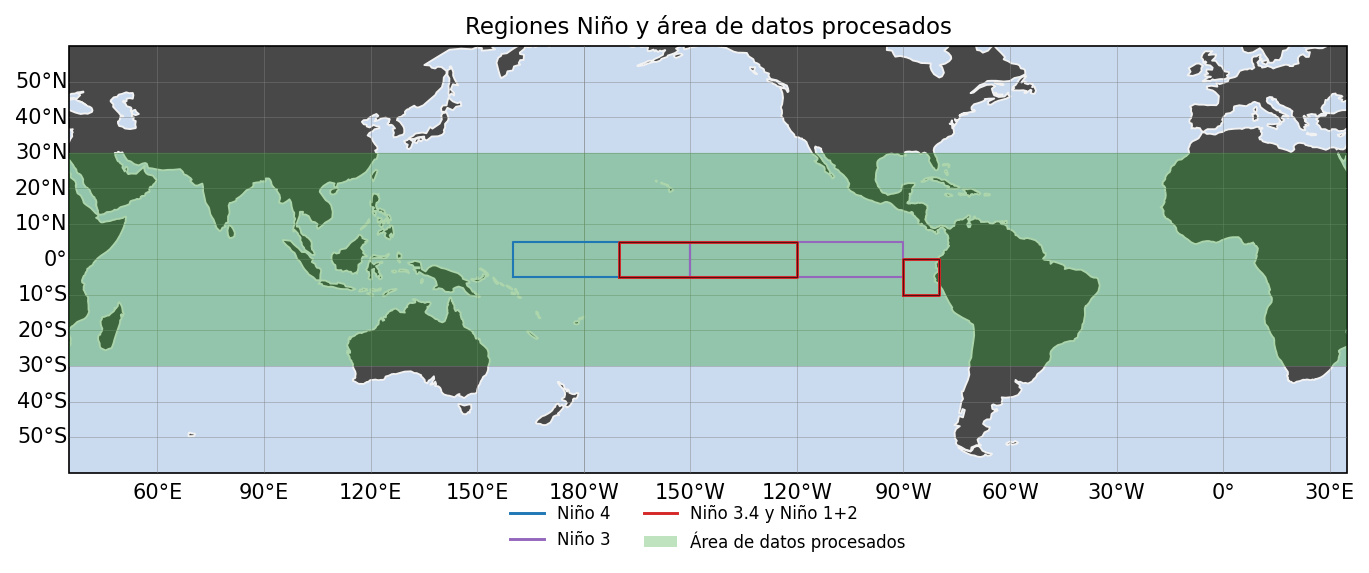
\includegraphics[width=0.9\textwidth]{figuras/region_nino_proj.png}
\caption[Ubicación de las cajas Niño~3.4 y Niño~1+2 y de la ventana de descarga.]{Regiones Niño~3.4 y Niño~1+2 (rojo), con Niño~4 y Niño~3 como referencia, en proyección cilíndrica centrada en Niño~3.4. El área verde es la ventana de descarga (0°--360°, 30°S--30°N): el dominio descargado, regrillado y enmascarado por el \emph{pipeline}. Niño~1+2, junto a la costa peruana y a la surgencia de la Corriente de Humboldt, es la caja de mayor relevancia para el monitoreo del Niño costero \citep{takahashi2019}; Niño~3.4 es la caja de referencia internacional del Índice Oceánico de El Niño (ONI).}
\label{fig:region_nino}
\end{figure}

La ventana cubre toda la franja tropical, y no solo el Pacífico, porque dos cálculos de los entregables siguientes necesitan la TSM media tropical de las tres cuencas: el índice RONI, que expresa la anomalía de Niño~3.4 relativa al promedio tropical, y el índice de calentamiento tropical del método ToD (Sección~\ref{sec:toe_metodos}). Descargar la franja completa en esta etapa evita descargas adicionales en los entregables siguientes.

Los periodos, definidos en \texttt{config/periods.yaml}, son: referencia y validación 1981--2014; proyección 2036--2065 (P1) y 2071--2100 (P2). El rango completo de descarga es 1850--2100 (\texttt{historical}: 1850--2014; escenarios SSP: 2015--2100). Los escenarios son \texttt{ssp245} y \texttt{ssp585}, más \texttt{ssp370} como escenario intermedio para el análisis de sensibilidad entre ambos. El único criterio de selección es la disponibilidad de \texttt{tos}/\texttt{Omon} en los cuatro experimentos.

\end{propuesto}

\bibliographystyle{plainnat}
\bibliography{../informe/references_rev}
\end{document}
